% Master document for the BSc APM thesis.
%
% SPDX-License-Identifier: GPL-3.0-or-later
% Copyright (c) BSc APM Case Study 2025-2026
%
% Single source of truth: this file sets the class, metadata, and shared
% preamble, then assembles the thesis from one body file per chapter under
% chapters/. Build from the repository root with `latexmk thesis.tex`
% See latexmkrc

\documentclass[ack]{apmthesis}

% Packages every chapter body may rely on. The class already provides
% graphicx, tabularx, longtable, and caption; the rest live here so chapter
% bodies stay preamble-free and are driven entirely by this master.
\usepackage{amsmath}
\usepackage{amssymb}
\usepackage{booktabs}
\usepackage{float}
\usepackage{threeparttable}
\usepackage{enumitem}
\usepackage{listings}
\usepackage{xcolor}
\usepackage[bottom,flushmargin]{footmisc}
\usepackage{hyperref}
\usepackage{xurl}
\usepackage{todonotes}
\newcommand{\ethan}[1]{\todo{@Thanassis:~#1}}
\newcommand{\me}[1]{\todo[inline,color=green!40]{@ me:~#1}}


\hypersetup{
  unicode=true,
  colorlinks=true,
  linkcolor=blue,
  citecolor=blue,
  urlcolor=blue,
  pdftitle={Agentic Project Management: A Spec-Driven Multi-Agent Framework for AI-Assisted Software Engineering}
}

% Code-listing style for any verbatim blocks
\lstset{
  basicstyle=\ttfamily\small,
  breaklines=true,
  frame=single,
  numbers=left,
  numberstyle=\tiny,
  stepnumber=1,
  tabsize=2
}

% IEEE reference style, resolved by biber. Identifiers print as plain text, and
% the author-list bounds are pinned because the style's defaults vary by release.
\usepackage[backend=biber,style=ieee,doi=true,isbn=true,url=false,
            hyperref=false,maxnames=6,minnames=3]{biblatex}
\addbibresource{references.bib}
\ExecuteBibliographyOptions[software]{url=true}

\newcommand{\placeholder}[1]{\textcolor{red}{\textit{[#1]}}}
\makeatletter
\newcommand{\InputTableRows}[1]{\@@input #1 }
\makeatother

\titleEn{Agentic Project Management: A Spec-Driven Multi-Agent Framework for AI-Assisted Software Engineering}
\titleGr{Agentic Project Management: Ένα Πολυπρακτορικό Πλαίσιο Οδηγούμενο από Προδιαγραφές για Ανάπτυξη Λογισμικού με Υποστήριξη Τεχνητής Νοημοσύνης}

\authorFirstEn{Konstantinos}
\authorFirstAbrEn{K.}
\authorMiddleEn{}
\authorLastEn{Chaidemenos}
\authorFirstGr{Κωνσταντίνος}
\authorFirstAbrGr{Κ.}
\authorMiddleGr{}
\authorLastGr{Χαϊδεμένος}
\authorSn{1115202200262}

\dateEn{AUGUST 2026}
\dateGr{ΑΥΓΟΥΣΤΟΣ 2026}

\supervisorEn{Thanassis Avgerinos}{Assistant Professor}
\supervisorGr{Θανάσης Αυγερινός}{Επίκουρος Καθηγητής}

\abstractEn{Coding agents now carry out substantial software tasks with limited direction from the developer. As a task grows, the agent must hold the project's intent while accumulating context competes for the model's finite attention. Recent solutions address this by recording intent in persistent documents and by dividing work among multiple agents.

We present Agentic Project Management (APM), an open-source framework that operates on top of interactive coding agents. APM combines persistent planning documents with role-specific division of work, and makes its coordination user-mediated: its agents communicate through the developer, allowing them to review and intervene as needed before passing each message on. The design aims to keep authority and decision-making over development with the user.

We evaluate APM against GitHub's Spec-kit through a within-participant case study where twelve developers each completed the same demanding task across two sessions, once with each framework, on Claude Code with Claude Opus 4.7 or Claude Sonnet 4.6. The comparison covers economic cost, each session's temporal and interaction shape, functional test scores, and developer perception. The frameworks carried no firm difference in functional outcome across the cohort, while APM's structure provided more stability under Sonnet. In exchange, APM took longer in all twelve pairs, adding a median of 36 minutes to session duration, and cost more in nine of the twelve pairs, adding a median of \$6.10 across the cohort, with the higher cost concentrated under Opus. Eleven of the twelve participants rated APM higher on effectiveness and nine on confidence. The study provides a reproducible methodology for evaluating this class of frameworks, while establishing the empirical trade-off of user-mediated coordination, which exchanges session duration and token expenditure for developer agency and review opportunities.}
\abstractGr{Οι πράκτορες προγραμματισμού αναλαμβάνουν πλέον σύνθετες εργασίες λογισμικού με ελάχιστη καθοδήγηση από τον προγραμματιστή. Όσο μια εργασία μεγαλώνει, ο πράκτορας καλείται να διατηρήσει την πρόθεση του έργου ενώ η συσσώρευση πληροφοριών διεκδικεί την πεπερασμένη προσοχή του μοντέλου. Πρόσφατες λύσεις αντιμετωπίζουν αυτό το ζήτημα καταγράφοντας την πρόθεση σε μόνιμα έγγραφα και μοιράζοντας την εργασία σε πολλαπλούς πράκτορες.

Παρουσιάζουμε το Agentic Project Management (APM), ένα πλαίσιο ανοικτού κώδικα που λειτουργεί πάνω από διαδραστικούς πράκτορες προγραμματισμού. Το APM συνδυάζει μόνιμα έγγραφα σχεδιασμού με κατανομή εργασίας σε διακριτούς ρόλους, και καθιστά τον συντονισμό διαμεσολαβούμενο από τον χρήστη: οι πράκτορές του επικοινωνούν μέσω του προγραμματιστή, επιτρέποντάς του να εξετάζει και να παρεμβαίνει όπως απαιτείται πριν προωθήσει κάθε μήνυμα. Στόχος του σχεδιασμού είναι να διατηρηθεί ο έλεγχος και η λήψη αποφάσεων στα χέρια του χρήστη.

Αξιολογούμε το APM έναντι του Spec-kit της GitHub μέσω μελέτης περίπτωσης όπου δώδεκα προγραμματιστές ολοκλήρωσαν την ίδια απαιτητική εργασία σε δύο συνεδρίες, μία με κάθε εργαλείο, στο Claude Code με τα μοντέλα Claude Opus 4.7 ή Claude Sonnet 4.6. Η σύγκριση καλύπτει το οικονομικό κόστος, τη χρονική και διαδραστική μορφή κάθε συνεδρίας, τη βαθμολογία σε λειτουργικούς ελέγχους και την αντίληψη των συμμετεχόντων. Δεν προέκυψε σαφής διαφορά στο λειτουργικό αποτέλεσμα στο σύνολο του δείγματος, ενώ η δομή του APM προσέφερε μεγαλύτερη σταθερότητα υπό το Sonnet. Σε αντάλλαγμα, το APM διήρκεσε περισσότερο και στα δώδεκα ζεύγη, προσθέτοντας διάμεσο χρόνο 36 λεπτών στη διάρκεια της συνεδρίας, και κόστισε περισσότερο σε εννέα από τα δώδεκα ζεύγη, προσθέτοντας διάμεση διαφορά 6,10 δολαρίων στο σύνολο του δείγματος, με το υψηλότερο κόστος να συγκεντρώνεται υπό το Opus. Παρ' όλα αυτά, έντεκα από τους δώδεκα συμμετέχοντες βαθμολόγησαν το APM υψηλότερα ως προς την αποτελεσματικότητα και εννέα ως προς την εμπιστοσύνη τους. Η μελέτη παρέχει μια αναπαραγώγιμη μεθοδολογία για την αξιολόγηση αυτής της κατηγορίας πλαισίων, τεκμηριώνοντας παράλληλα τον εμπειρικό συμβιβασμό του διαμεσολαβούμενου από τον χρήστη συντονισμού, που ανταλλάσσει χρονική διάρκεια και υπολογιστικό κόστος με ανθρώπινο έλεγχο και ευκαιρίες επισκόπησης.}
\acksEn{To my parents, my loved ones, and all the people who stood by me during this challenging effort.

I also thank my supervisor for the guidance that shaped this work, and the twelve participants who gave their time to the study.}

\subjectAreaEn{Software Engineering}
\subjectAreaGr{Τεχνολογία Λογισμικού}
\keywordsEn{agentic project management, coding agents, multi-agent systems, spec-driven development, AI-assisted software engineering, case study}
\keywordsGr{agentic project management, πράκτορες προγραμματισμού, πολυπρακτορικά συστήματα, ανάπτυξη οδηγούμενη από προδιαγραφές, τεχνητή νοημοσύνη στην ανάπτυξη λογισμικού, μελέτη περίπτωσης}

\begin{document}

\frontmatter

\me{On the abstracts and Introduction, I added findings using Evaluation Methodology's terminology. I think Introduction already broadly followed your five-paragraph suggestion, so I mainly restructured and rephrased it. I hope it now meets the standard you had in mind. I also made methodology the second contribution, named its intended users, and aligned chapter names and references.}

\me{On moving definitions into Background, I prefer each chapter to introduce the concepts later ones need and build on the vocabulary established earlier. Therefore: Background supplies broad field concepts that will be used throughout all the other chapters; APM's Design adds framework terms used in the evaluation and the findings; Evaluation Methodology adds study terms, metrics and statistics. My aim is to define each term on first use and let later chapters build on it. I'm unsure whether this conflicts with any academic convention; I think it is broadly consistent with academic writing and reads well, though it is a personal preference. Moving these definitions back to Background would, I think, upset the current chapter balance and make it read more like a glossary.}

\me{On Background specifically, it additionally establishes the related work and the research gap alongside establishing its concepts. This is intentional but only my preference: I think it reads better. I also incorporated the student study you suggested and replaced source-only footnotes with citations. (I did this throughout the thesis. As a result we now have, including the new additions, 51 distinct cited sources, up from about 20. I only retained substantive remarks as footnotes.) I kept the gap comparison in prose instead of adding a checklist as you suggested, because I think it would imply a ranking and read less smoothly going against the rest of the thesis conventions.}

\me{On the metric headings, I prefer the same four dimension names in Evaluation Methodology and Evaluation Results. Matching the definitions to their results this way makes the comparison easier to map and easier to follow, I think. This is also a personal preference. I like concise headings.}

\me{On using the academic 'we', I retained 'the author' only for APM's independent origins, to not suggest that APM was conceived in a controlled or supervised environment. I used ``we'' throughout the thesis for everything else, like the specific APM version that is presented and the evaluation methodology etc. I'm unsure whether this distinction follows the preferred convention, please let me know.}

\me{On APM's overview, I added Section~\ref{sec:framework-design-overview} and reorganised APM's Design (previously Framework Design) around Agent Roles, Agent Coordination, State Management, and Project Management (previously Workflow Overview, now details the specific project management aspects of the framework). I kept the overview broad and plain: its purpose is to give the big picture and host two new high-level workflow diagrams before any detailed mechanics. I used a different diagram style for these, draw.io with Lucide icons, and also applied to the rest that depict specifc mechanisms of the workflow. Only the Project Management diagrams stay in declarative D2 diagramming. I addressed all the smaller wording and definition notes. Two specific clarifications: the user mediates exchanges and can interrupt running work while the Manager waits for its report. Interrupted work returns with analogous information to the Manager. It is asynchronous. I could not think of a useful OS analogy. Workers don't need a wider view of the Plan. I had omitted an existing mechanism from the description. The Manager's Task Prompts supply relevant planning, upstream, and downstream context according to the Task. It preserves scoped context while providing any part of the wider picture as needed. No need to add anything for this to Future Work.}

\me{On the new reflection citations, I placed one sentence in APM's Design to show that earlier work in human–computer and human–AI interaction has explored a related idea. APM was developed independently; these papers neither motivated its design nor establish that its review points improve reflection.}

\me{On choosing Spec-kit, I added the rationale in Section~\ref{sec:evaluation-comparison-framework}: it is another framework of the same class, with a spec-driven workflow but different coordination. I kept its account in Evaluation Methodology, after APM's Design, for the reason I explained above about concept definition ownership etc. I think GitHub's authorship gives Spec-kit enough credibility, but does not justify calling it ``state of the art''. I would instead present it as a recognisable spec-driven comparator with a different approach to coordination. I also added an unguided-agent baseline to Future Work.}

\me{On the methodology contribution, I separated the setting into Case-Study Conditions and made the open-source task package and the AI agent setup helper explicit parts of it.}

\me{On what grading checks, I clarified that it is deterministic and limited to task-required MCP behaviour. No need to clarify that it is NOT LLM-based/neural etc. It establishes neither full protocol compliance, only checks the MCP protocol surface that the task requires, nor code quality, just the running behaviour. I would avoid LLM bug counts because they depend on the judging model and conflict with the deterministic approach I wanted for the evaluation and APM's presented 'ideology'.}

\me{On cost, I clarified that I compute it deterministically afterwards from each conversation's Claude Code JSONL transcript, pricing recorded token usage per API call, including cache reads and writes, against the relevant model's rate card.}

\me{On confidence intervals, I added textbook references in Section~\ref{sec:evaluation-analysis-plan}, including a worked small-sample interval. They support an established procedure, rather than a ``gold standard''. I favour its exact reference calculation over a large-sample approximation, but it still assumes independent, symmetric paired differences. The stated coverage is calibrated for continuous data; ties can make it conservative. I would keep the intervals: they often inform findings the summary values alone would miss. I removed repeated coverage percentages from captions.}

\me{On the functional-score pattern favouring APM under Sonnet, I highlighted it in the abstracts but would keep the interpretation within this study given the small group. I would keep that reading descriptive: the model groups contain different participants, and a few blocking failures, which we also examine further in Section~\ref{sec:discussions-blackbox}, strongly affect the scores.}

\me{On developer understanding, I agree that felt confidence and control leave comprehension and exercised authority unmeasured. I made task ownership an explicit limit in Discussion and developed the understanding question in Future Work, with sources on AI-generated code quality and comprehension exercises. I also reorganised Future Work into separate investigations. I think it reads more clearly now, identifying benefits the current study cannot establish.}

\mainmatter

\chapter{INTRODUCTION}
% Introduction chapter body. Included by thesis.tex under \chapter{INTRODUCTION}.

\placeholder{Forthcoming. Problem (context decay, the limits of single-agent
AI coding on complex software); the proposition (structured multi-agent
coordination); the claim and how a controlled comparative case study against a
single-agent spec-driven baseline supports it; a Summary of Contributions; a
Thesis Structure section.}


\chapter{BACKGROUND}
\label{chap:background}
% Background chapter body. Included by thesis.tex under \chapter{BACKGROUND}.

\section{AI Coding Assistants and the Agentic Model}
\label{sec:coding-assistants}

How developers work with AI has changed quickly, from tools that completed a line of code to systems that carry out whole programming tasks on their own. The earliest of these were predictive. Integrated development environments have offered identifier and interface completion since the 1990s, and by the late 2010s those suggestions were ranked by machine-learning models trained on large code corpora. Such systems retrieve and rank symbols that already exist; they do not compose new code. The generative shift came when large language models (LLMs) trained on code began producing novel, multi-line completions inline in the editor, the form that GitHub Copilot brought to a wide audience in 2021.\footnote{GitHub Copilot technical preview, June 2021: \url{https://github.blog/2021-06-29-introducing-github-copilot-ai-pair-programmer/}.} A second and distinct mode of interaction followed in late 2022, when general-purpose conversational assistants reached the public. While these were not explicitly coding tools, developers used them broadly, to explain unfamiliar code, stand in for documentation, or think through a problem as much as to draft a snippet to paste back. This conversational mode was soon folded into the editor, and then extended past advice into action. The assistant started editing files, running commands, and revising its work against the results. Tools of this last kind, which act on a project rather than only commenting on it, are called \emph{agentic}; they emerged over 2024 and 2025.\footnote{Early examples include Devin, announced in March 2024 as an autonomous ``AI software engineer'' acting on a project from its own sandboxed environment rather than the developer's editor (\url{https://www.cognition.ai/blog/introducing-devin}), and GitHub Copilot's agent mode, introduced in February 2025, which works inside the editor to plan a task, edit across multiple files, run commands, and iterate on the results (\url{https://code.visualstudio.com/blogs/2025/02/24/introducing-copilot-agent-mode}).} It is this conversational line, rather than inline completion, that the agentic systems studied in this thesis descend from.

We use the term \emph{agent} in a specific sense throughout this thesis. In its classical formulation, an agent is anything that perceives its environment through sensors and acts upon that environment through actuators \cite{russell2021aima}. Brought into the setting of LLMs, an agent is built around an LLM, with the ability to perceive and use external tools and resources, extending it beyond producing text into planning, memory, and action \cite{liu2024llmagents}. What distinguishes such an agent from a fixed program is where control of the process sits. An agent directs its own steps and tool use, choosing what to do next, whereas a workflow drives the model along predefined paths \cite{anthropic2024agents}. The frameworks evaluated in this thesis are agentic in precisely this sense, the model rather than a fixed script driving the work.

The effect of these tools on developer productivity is measured, and contested, and the evidence spans different generations of the technology. Field experiments with an earlier generation of assistant reported substantial gains. In three randomised controlled trials run at Microsoft, Accenture, and a Fortune-100 company, several thousand professional developers given an AI coding assistant completed around a quarter more tasks, with the clearest gains among the less experienced \cite{cui2026genai}. Evidence from agentic tools points the opposite way. In a trial run by METR in early 2025, with the Cursor editor\footnote{Cursor, an AI code editor: \url{https://cursor.com}.} driving Claude 3.5 and 3.7 Sonnet, experienced open-source maintainers working on their own repositories were left roughly 19\% slower, even as those same developers expected to be sped up \cite{becker2025metr}. The two studies differ in their tools, their tasks, and the developers they observed, so the effect reads as conditional rather than settled. Both, like the wider productivity literature, ask only whether AI assistance helps; neither varies the workflow or framework through which a developer works with the agent, which is the dimension this thesis sets out to compare.

\section{Context Windows and Context Decay}
\label{sec:context-windows}

Whatever its form, an agent operates within a context window: the bounded span of tokens the underlying model can attend to at once. Into it go the system prompt, the instructions the agent was given, the files and tool output it has read, and its own earlier turns; a long task steadily fills it. A frontier model's context window now spans several hundred thousand to a million tokens, yet even that can be too small to hold an entire repository and run a complex task end to end.

A model does not even use the context it has evenly. Controlled experiments on long-context models found a U-shaped pattern in which performance is highest when the relevant information sits at the start or the end of the input and falls sharply when it lands in the middle, even for models built for long contexts \cite{nliu2023lostmiddle}. Usable capacity is therefore smaller than the raw token count suggests.

For an agentic coding session the consequence is direct. As the session runs, every file read, tool called, and command executed consumes context. As that context fills, the agent is more likely to forget earlier decisions, lose track of completed work, or drift from the original goal \cite{liu2024llmagents}. Summarising earlier context or retrieving it on demand buys room, but only by discarding detail, trading fidelity for space.

This accumulation also carries a direct monetary cost. Each step is produced by running the model over the entire session so far, supplied to it as input, and a call is priced by the number of tokens it processes. Every step therefore costs more than the one before it, and the cumulative cost of a long task grows faster than the number of steps it takes \cite{gao2025turncontrol}.

\placeholder{Forthcoming. Spec-driven development and its single-agent
reference implementation; single- versus multi-agent coordination; and a
compact positioning of the gap this thesis addresses.}


\chapter{APM'S DESIGN}
\label{chap:framework-design}
% !TEX root = ../../thesis.tex
% Framework Design chapter body. Included by thesis.tex under
% \chapter{FRAMEWORK DESIGN}.

\section{Design Goals}
\label{sec:framework-design-goals}

APM is a MAS intended for substantial, real-world software projects. It limits context accumulation by dividing a project across separate agent conversations. Because this also separates knowledge and decisions, the agents use shared project information to keep their contributions consistent with what they should collectively produce.

APM gives each agent a distinct responsibility. One handles planning, producing a durable account of what to build and how to build it. During implementation, agents carry out bounded parts of it under an agent that coordinates their execution. The coordinating agent maintains the project-wide view, distributes and reviews work, and preserves coherence as implementation proceeds.

Shared files enable this division. They hold project intent, execution state, and information exchanged among agents, while explicit protocols define what each agent reads and writes. Documents authored during planning provide implementation with a durable reference to what the project must produce and how it is organised. Detailed execution history is reduced to records containing the outcomes and observations that coordination requires. These files are shared across conversations and persist beyond any one of them, preserving the knowledge and decisions needed for continuity.

APM deliberately brings human involvement into how the project is developed and how its agents interact. Each agent runs in a conversation directly addressable by the user, who carries the communication between them and holds final authority over project decisions. Review points keep planning, coordination, and execution visible and open to intervention.


\chapter{EVALUATION METHODOLOGY}
\label{chap:evaluation-methodology}
\documentclass[11pt, a4paper]{article}

% ============================================================================
% PACKAGES
% ============================================================================
\usepackage[T1]{fontenc}
\usepackage[utf8]{inputenc}
\usepackage[margin=1in]{geometry}
\usepackage{amsmath}
\usepackage{amssymb}
\usepackage{graphicx}
\usepackage{booktabs}   % For professional looking tables
\usepackage{tabularx}   % For flexible table widths
\usepackage{hyperref}   % For links
\usepackage{xcolor}     % For placeholder text
\usepackage{titlesec}
\usepackage{enumitem}
\usepackage{caption}
\usepackage[bottom,flushmargin]{footmisc}  % Pin footnotes to page bottom, flush left

% ============================================================================
% CONFIGURATION
% ============================================================================
\hypersetup{
    colorlinks=true,
    linkcolor=blue,
    citecolor=blue,
    urlcolor=blue
}

% Placeholder command for easy visual identification
\newcommand{\placeholder}[1]{\textcolor{red}{\textit{[#1]}}}

% Line spacing
\renewcommand{\baselinestretch}{1.15}

% Paragraph formatting: no indent, vertical separation between paragraphs
\setlength{\parindent}{0pt}
\setlength{\parskip}{0.5\baselineskip}

% Allow a small amount of extra inter-word stretch as a last resort when
% breaking paragraphs, to avoid minor overfull boxes in dense prose.
\setlength{\emergencystretch}{3em}

\begin{document}

% ============================================================================
% EVALUATION SECTION
% ============================================================================

\section{Evaluation Methodology}
\label{sec:evaluation}

This chapter details the methodology used to evaluate the Agentic Project Management (APM) framework. To assess the framework in a realistic setting, we conducted a comparative case study involving human participants. The study compares APM, a multi-agent framework that distributes work across specialised agents, against GitHub Spec-kit, a single-agent toolkit that guides one AI agent through a structured specification-driven workflow. Both frameworks are described in Section~\ref{sec:frameworks}. The study was conducted in May 2026 on the Claude Code command-line interface; pricing, model, and command-set statements in this chapter refer to that snapshot.

The evaluation measures three distinct dimensions:

\begin{itemize}
    \item Economic Efficiency (dollar cost of a session, computed against the platform's per-token rate card)
    \item Process Efficiency (human cognitive load and interaction burden across a session)
    \item Functional Efficacy (ability to complete non-trivial tasks)
\end{itemize}

\subsection{Research Objectives}

The primary objective of this research is to determine whether the structural overhead introduced by APM, in the form of multi-agent orchestration and the explicit Planning and Implementation phases, produces measurable improvements over a single-agent workflow. This evaluation contributes a cost perspective alongside the process and functional dimensions.

We define the following Research Questions (RQs):

\begin{itemize}
    \item \textbf{RQ1 (Economic Efficiency):}
    \begin{itemize}
        \item Does APM's multi-agent coordination produce a measurably different dollar cost per session than Spec-kit's single-agent workflow?
        \item Where in each framework's workflow does session cost concentrate between the planning phase and the implementation phase, and does that concentration pattern differ between frameworks?
        \item Does cumulative session cost comparison between the two frameworks shift, when using models with different context-window capacities and capabilities?
    \end{itemize}
    \item \textbf{RQ2 (Process Efficiency):}
    \begin{itemize}
        \item Does APM's structure reduce the amount of manual effort the user must invest during execution, particularly interventions, corrections, and clarifications?
        \item If a difference in user effort is observed, is it significant enough to justify the structural overhead APM introduces?
        \item Given that the user remains in the loop as a message carrier, can the agents coordinate effectively enough that the user's role can be limited to shuttling messages rather than correcting or redirecting agent behaviour?
    \end{itemize}
    \item \textbf{RQ3 (Functional Efficacy):}
    \begin{itemize}
        \item Can APM successfully deliver complex, non-trivial features in scenarios where single-agent workflows are prone to failure due to context window exhaustion, loss of coherence across long sessions, or inability to coordinate work across multiple concerns?
        \item How does the performance of APM compare to the performance of a single-agent workflow?
    \end{itemize}
\end{itemize}

\subsection{Frameworks Under Evaluation}
\label{sec:frameworks}

The two frameworks are both open-source and spec-driven, running on the same AI coding CLI. Both structure work through explicit specification and planning artifacts before implementation begins. They differ in how execution is organised: Spec-kit operates within a single agent conversation, while APM distributes work across multiple specialised agents.

\subsubsection{GitHub Spec-kit}

Spec-kit\footnote{Documentation available at: \url{https://github.github.com/spec-kit/}} is a specification-driven development toolkit developed by GitHub. It guides a single AI agent through a structured workflow using three sequential commands:

\begin{enumerate}
    \item \texttt{/speckit-specify}: transforms a feature description into a structured specification containing requirements, user stories, and acceptance criteria.
    \item \texttt{/speckit-plan}: converts the specification into a technical implementation plan with architecture decisions, data models, API contracts, and supporting documents.
    \item \texttt{/speckit-tasks}: derives an executable task list (\texttt{tasks.md}) from the plan, with parallelism annotations and sequencing constraints.
\end{enumerate}

Execution is triggered by a fourth command, \texttt{/speckit-implement}, which parses the task list and carries out each task in sequence. Additional commands support iterative refinement (\texttt{/speckit-clarify}), cross-artifact consistency checking (\texttt{/speckit-analyze}), and custom quality checklists (\texttt{/speckit-checklist}). A constitution mechanism, maintained via the \texttt{/speckit-constitution} command, allows users to establish architectural rules that the agent enforces throughout the workflow.

All planning and implementation happens within one continuous conversation. The agent acts as both planner and executor, and the full specification, plan, and task context accumulates in a single context window. Spec-kit produces a fixed set of artifact types (specification, plan, data model, contracts, research, tasks) regardless of project type; the templates are predefined and every project receives the same artifact layout.

\subsubsection{APM in Comparison}

Where Spec-kit runs the entire workflow in a single conversation, APM separates planning, coordination, and execution across three agent roles, each operating in its own conversation with scoped context. Agents communicate through a file-based Message Bus; planning documents adapt to each project rather than conforming to a predetermined artifact layout; and the user acts as a message carrier between conversations. When an agent's context fills, a Handoff mechanism preserves working knowledge across conversations.

\subsection{Testbed and Task Design}

To evaluate the frameworks under realistic constraints, we used an existing open-source project, the \texttt{eclass-mcp-server},\footnote{Repository available at: \url{https://github.com/sdi2200262/eclass-mcp-server}} a Python-based Model Context Protocol (MCP)\footnote{Protocol specification available at: \url{https://modelcontextprotocol.io}} server designed to interface with the \texttt{openeclass} platform.\footnote{Repository available at: \url{https://github.com/gunet/openeclass}} Openeclass is an online platform for Greek universities that allows students to manage their courses and assignments.

\subsubsection{Task Description}

The task requires participants to implement two new announcement tools in the Python MCP server and to create a complete native C replica of the entire server with some explicit strict constraints.\footnote{\raggedright Task specification, participant package, and containerised testing environment available at: \url{https://github.com/sdi2200262/bsc-apm-case-study-task}} The two tools are:

\begin{itemize}
    \item \texttt{get\_course\_announcements}: retrieves announcements for a specific course.
    \item \texttt{get\_general\_announcements}: aggregates system-wide and per-course announcements.
\end{itemize}

The C implementation adds significant complexity: participants must manage code translation, memory safety, and protocol details across two different languages. The combination of feature implementation and full-language replication is designed to challenge the two frameworks and expose any differences between them, particularly when context window limits become a bottleneck.

The task admits more than one viable implementation path; a scoring rubric\footnote{\raggedright Scoring rubric and grading infrastructure available at: \url{https://github.com/sdi2200262/bsc-apm-case-study-infra}} awards points to any path that meets its per-test specifications.

\subsubsection{Task Environment}
\label{sec:task-env}

Each session runs in a workspace prepared up-front. The working directory is a fresh clone of \texttt{eclass-mcp-server} checked out to a fixed patch-baseline commit against which the participant implements the task; the submission patch is the diff between this baseline and the participant's staged changes. A read-only reference clone of \texttt{openeclass} at a fixed inspection commit is also present, so any research the assistant performs into the legacy server's source reads from a fixed snapshot rather than a moving target. Alongside the workspace runs a containerised mock of the openeclass platform; the mock is built from that same inspection commit, only compiled, seeded with deterministic fixture data, and packaged in a Docker image, and paired with a deterministic mock single-sign-on service. The assistant therefore inspects the very source that the running mock executes.

The mock is the participant's integration target during development and the same target the grader replays when scoring, so every cohort participant develops and is graded against the same fixed state of the platform. The exact pins, the upstream release tag the image is built from, the seeded fixtures, and the mock authentication surface are documented in the Reference Environments subsection of the Evaluation Appendix.

\subsection{Study Design}
\label{sec:study-design}

The study compares the two frameworks across a homogeneous cohort of participants drawn from University students and working professionals. The design is within-subjects: every participant contributes data points for both frameworks, so per-participant variance in skill, prior experience, and working style is absorbed into each pairwise comparison rather than confounding it.

\subsubsection{Counterbalancing}
\label{sec:counterbalancing}

Each participant completes the case study task twice, once with APM and once with Spec-kit, each session time-boxed to a maximum of three hours. Two factors are counterbalanced across the cohort: the framework order and the model assignment.

The framework-order factor varies which framework a participant encounters first. Counterbalancing the order lets any observed first-to-second-session improvement be attributed to task familiarity rather than to the framework itself; the resulting first-to-second-session learning is analysed in the Learning Effects subsection in Section~\ref{sec:results}. The model factor varies which Claude model drives both of a participant's sessions, held fixed within the participant. Each participant is assigned one of Claude Opus 4.7 and Claude Sonnet 4.6. The two models differ in capabilities and context-window capacity, one million tokens for Opus 4.7 against two hundred thousand for Sonnet 4.6.

The cohort is split across four assignment cells: APM first with Opus, Spec-kit first with Opus, APM first with Sonnet, and Spec-kit first with Sonnet. Holding the model fixed within participant lets the within-participant framework comparison absorb the model factor into the participant's own variance; the cohort-level analysis additionally compares the framework effect across the two models.

The two sessions are isolated from one another so that no code, workspace state, or assistant context from the first session can influence the second. The full session-isolation procedure is documented in the Submission Workflow subsection of the Evaluation Appendix.

\subsubsection{Data Source}
\label{sec:data-source}

Each session produces a participant submission composed of three artefacts: a solution patch the participant writes against the patch baseline, the set of Claude Code JSONL transcripts the CLI persists for every conversation opened during the session, and a post-session questionnaire response.

The solution patch is the participant's functional contribution and the input to scoring. The transcripts are the source of every cost, time, message-activity, and reliability measurement: each transcript provides a structured record of every conversation, so the measurements are extracted programmatically rather than by manual annotation. Auxiliary records that Claude Code persists for any subagents the conversation dispatched and for any tool results it offloaded from the main file travel with the transcripts, so a complete record of the session is available for measurement.

The post-session questionnaire complements the transcript-derived measurements with self-reported workload and perception items and is submitted alongside the patch and the transcripts through a single per-session combined web form. Its captured items and response scale are documented in the Post-Session Questionnaire Instrument subsection of the Evaluation Appendix.

Participant data is anonymised and encrypted before storage; the sanitisation scheme is documented in the Data Privacy and Sanitisation subsection of the Evaluation Appendix.

\subsection{Metrics}
\label{sec:metrics}

Every measurement defined in this section is extracted from the participant's submission by the same procedure across the cohort. The economic, process, and supplementary measurements are derived from the session's transcripts; the functional measurements are derived from the solution patch, scored against the rubric introduced earlier.

Every transcript-derived measurement is computed at two scopes per submission, per-session and per-phase, where the phases are the planning portion and the implementation portion of the session. A third per-role scope is emitted explicitly for APM submissions, splitting the session by Planner, Manager, and Worker.

Per-session is the headline scope on which the two frameworks are compared, since it places APM's multi-conversation workflow and Spec-kit's single conversation on the same denominator. Per-phase and per-role views locate where within a session each framework spends its budget and effort. Phase boundaries and APM roles are detected automatically; the detection rules are documented in the APM Role Detection and  Framework Phase Detection subsections of the Evaluation Appendix. The functional dimension admits no phase or role decomposition and is reported per submission only.

Each measurement carries an anchor flag distinguishing Primary measures (those that drive a research question and enter hypothesis testing), Secondary measures (those that decompose or support a Primary), and Supplementary measures (descriptive only). The subsections below specify each measurement dimension one by one.

\subsubsection{Economic}

The primary economic measurement is the \textbf{dollar-equivalent cost}, computed by pricing every call recorded in the session's transcripts against Anthropic's published per-token rate card at the study's snapshot date, across the five token categories the rate card specifies. Calls made by the conversation's primary agent are priced at that conversation's declared model; calls made by subagents are priced against the model recorded in the platform's sibling subagent transcript for that dispatch.

A session's cost is reported as a point estimate when every dispatch resolves to a single model and as lower and upper bounds when a dispatch's model cannot be determined deterministically. The full attribution rules, the fallback resolution path, and the bracketing scheme are documented in the Per-Token Rate Card subsection of the Evaluation Appendix.

Each participant contributes one APM cost and one Spec-kit cost for the same task, compared pairwise across the cohort at the per-session scope.

\subsubsection{Process}

The process metrics capture the burden each framework imposes on the user across a session and are separated into how the user interacted with the model and how they invested their time during the session.

User-message activity is partitioned along two dimensions. The first is the kind of message the user typed:
\begin{itemize}
    \item \textbf{turn prompts} are prompts submitted while the agent was idle, opening a new turn.Each turn is the wall-clock interval from a user prompt to the assistant's idle return.
    \item \textbf{steers} are interjections enqueued while the agent was still working, which the platform either delivers to the agent during the turn or abandons if the user retracts them before delivery. Steer activity is additionally reported as three counts: \textbf{steer attempted}, \textbf{steer delivered}, and \textbf{steer abandoned}.

\end{itemize}

Each prompt and each delivered steer is assigned to one of three buckets along the second dimension:
\begin{itemize}
    \item \textbf{short} for brief acknowledgments or routing messages.
    \item \textbf{protocol} for framework-protocol messages such as APM or Spec-kit slash-command invocations.
    \item \textbf{standard} for substantive task-related prompts.
\end{itemize}

The \textbf{bucket-share distribution} reports the share of each bucket in the session's total user-message count, separately for prompts and for delivered steers and jointly across both; \textbf{magnitude per bucket} reports the mean character count of messages in each bucket. Together these views expose whether a framework's user burden is concentrated in mechanical message-shuttling (high protocol share, low magnitude) or in substantive corrections and guidance (high standard share, high magnitude).

The temporal shape of the session is captured by a family of turn-time metrics:
\begin{itemize}
    \item \textbf{session duration} is the wall-clock time from the first user message of the session to the last assistant message, bounded above by the three-hour cap.
    \item \textbf{turn count} is the number of turns recorded across the session's conversations.
    \item \textbf{mean turn duration} is the average turn-time, complemented by the \textbf{median}, the \textbf{ninety-fifth percentile}, and the \textbf{standard deviation} of the per-turn duration distribution.
    \item \textbf{turn time} is the wall-clock union of every turn's interval, reported in total and decomposed into the share spent in a single conversation at a time (\textbf{turn time solo}) and the share where two or more conversations were active simultaneously (\textbf{turn time concurrent}); for APM's multi-conversation design the decomposition surfaces whether the participant ran agents in parallel or serially.
    \item \textbf{inter-turn time} is the residual of the session duration once turn time has been subtracted: the wall-clock gap between consecutive turns, summed across the session. It is the assistant's idle time as recorded in the transcripts and is not interpreted as a measure of participant activity, since the participant may be reading, thinking, switching context, or away from the workstation during any gap.
\end{itemize}

Session duration, turn time with its solo and concurrent decomposition, and inter-turn time are reported at the per-session and per-phase scopes only; the wall-clock union and concurrency interpretations are not well-defined at role scope, where a role lives inside a single conversation file whose own turns cannot overlap.

\subsubsection{Functional}

The functional dimension scores each submission against the task's scoring rubric introduced earlier. The rubric is a fixed set of tests; each test checks one expected behaviour, produces a pass-or-fail verdict, and contributes a calibrated point weight to a 100-point total, so a submission that delivers only part of the task earns proportionally for what works.

The 100 points are split across the task's two implementations. The Python implementation carries 41 points: a baseline section that confirms the four pre-existing tools still work, and two feature sections covering the new course-announcement and general-announcement tools. The C replica carries 59 points: a build-and-stack section, a baseline section that re-implements the same four tools from scratch, the two announcement features mirrored against the C binary, and a memory-safety section exercised under Valgrind. The per-section point allocations, the per-test definitions, and the assertion logic each test uses are documented in the Test Suite Composition subsection of the Evaluation Appendix.

The primary functional outcomes are the total rubric score and the per-section scores: the first summarises the framework comparison in a single number, the second locates where each framework's work lands within the rubric.

\subsubsection{Supplementary}

A small set of supplementary descriptors is reported per framework alongside the primary and secondary measurements. They are descriptive only and do not enter the paired hypothesis testing.

The \textbf{tool success rate} is the proportion of every tool invocation result recorded on the session's main transcripts that does not carry an error flag, spanning every tool the assistant may invoke (file edits, shell, search, web fetches, MCP calls) without weighting by tool kind. Tool calls made inside subagent dispatches are not included. The rate is dominated by the underlying model's tool-use capability rather than by framework choice.

The \textbf{subagent dispatch count} is the number of \texttt{Task}-tool dispatches the main agent issued in scope, and the \textbf{delegated tool-use count} is the total number of tool invocations those dispatched subagents performed inside their own conversations. Together they characterise how much work each framework offloads to delegated subagents.

The \textbf{model-invoked Skill count} is the number of platform-rendered Skill bodies the agent itself caused to be injected through the Skill tool, surfacing self-invocation behaviour that does not appear in the user-message activity.

\subsubsection{Analysis Plan}
\label{sec:analysis-plan}

Each measurement is reported at the cohort level as a descriptive summary first (mean, standard deviation, median, and inter-quartile range per framework and per model band) and then as a paired framework comparison. The descriptive summaries report what a typical APM session and a typical Spec-kit session cost, take, and produce, and locate the spread of the cohort around those typical values. The paired comparison establishes whether the per-participant difference between the two frameworks is systematic across the cohort and how large that difference is relative to the per-participant variance.

The paired comparison uses a paired $t$-test on the per-participant difference. Given the two paired values $x_i^{\text{APM}}$ and $x_i^{\text{SK}}$ for participant~$i$, the difference $d_i = x_i^{\text{APM}} - x_i^{\text{SK}}$ has mean $\bar{d}$ and standard deviation $s_d$ across the cohort of $n$ participants; the test statistic is
\[
    t = \frac{\bar{d}}{s_d / \sqrt{n}},
\]
and the reported $p$-value comes from the two-sided $t$ distribution on $n - 1$ degrees of freedom.

The effect size is Cohen's $d_z$, the standardised mean difference in pooled within-pair-variance units,
\[
    d_z = \frac{\bar{d}}{s_d},
\]
which expresses the framework gap in standard deviations rather than in the metric's native units and so makes effect sizes comparable across metrics of different scale.

Every primary measurement is analysed this way: total rubric score, per-section scores, per-session cost, phase-broken cost shares, bucket-share distribution and magnitude per bucket across turn prompts and delivered steers, the turn-time decompositions, and session duration. The model factor is handled by stratification: paired comparisons are reported within each model band and then jointly across the cohort, exposing any framework effect that holds in one band but not the other.

Correlations between economic, process, and functional metrics are reported as Pearson coefficients within each framework and across the combined cohort. Pearson's $r$ is the standardised linear-association statistic on the pair $(x_i, y_i)$:
\[
    r = \frac{\sum_i (x_i - \bar{x})(y_i - \bar{y})}{\sqrt{\sum_i (x_i - \bar{x})^2 \, \sum_i (y_i - \bar{y})^2}},
\]
taking values in $[-1, 1]$. Correlation magnitudes are interpreted alongside the within-framework spread; they surface whether framework-induced variation in cost or process burden translates into functional outcomes.

Learning effects are analysed separately across the counterbalanced orderings. A learning-effect matrix reports mean first-to-second-session improvement across both framework orderings for each metric; an order-effect comparison between APM-first and Spec-kit-first directions tests whether the order of exposure affects the improvement; and the aggregate first-to-second-session improvement across orderings gives the baseline task-learning estimate.

% ============================================================================
% RESULTS
% ============================================================================

\section{Results}
\label{sec:results}

\subsection{Economic}

\placeholder{Forthcoming. Quantitative results for the per-session cost and the phase-broken decomposition. Tables: cohort-level descriptive summaries (mean, standard deviation, median, IQR) per framework and per model band; paired APM-versus-Spec-kit cost distributions stratified by model band and pooled across the cohort, with paired $t$-test statistics, $p$-values, and Cohen's $d_z$; planning-versus-implementation cost shares per framework; per-role cost shares across Planner, Manager, and Worker for the APM cohort; cost composition by token category and by main-versus-delegated population; Pearson correlations against rubric score within and across frameworks.}

\subsection{Process}

\placeholder{Forthcoming. Quantitative results for the user-burden metrics. Tables: bucket-share distribution and magnitude per bucket across turn prompts and delivered steers, paired across frameworks with $t$-statistics and Cohen's $d$; steer attempted, delivered, and abandoned counts per framework; turn-time decompositions (solo, concurrent, inter-turn) and the per-turn duration distribution; session-duration distributions against the three-hour cap; Pearson correlations against rubric score. Self-reported workload items from the post-session questionnaire are reported alongside the instrumented coordination metrics.}

\subsection{Functional}

\placeholder{Forthcoming. Quantitative results for the 100-point rubric. Tables: total-score distribution per framework, per-section score distributions across the Python and C implementations, per-test pass rates, baseline-regression rates, and paired framework comparisons with $t$-statistics and Cohen's $d$. Perceived framework effectiveness from the post-session questionnaire is reported alongside the rubric outcomes.}

\subsection{Supplementary}

\placeholder{Forthcoming. Descriptive per-framework summaries for the supplementary metrics: tool success rate, subagent dispatch count, delegated tool-use count, and model-invoked Skill count. Reported as cohort-level descriptives per framework and per model band without paired hypothesis testing.}

\subsection{Learning Effects}

\placeholder{Forthcoming. Quantitative results for the learning-effect analysis: first-to-second-session improvement matrix across framework orderings for functional, economic, and process metrics; order-effect comparison between APM-first and Spec-kit-first directions; and the aggregate baseline task-learning estimate across orderings.}

% ============================================================================
% DISCUSSION
% ============================================================================

\section{Discussion}
\label{sec:discussion}

\subsection{Economic Efficiency}
\label{sec:discussion-economic}

\placeholder{Forthcoming. Discussion of the per-session cost comparison, the phase-level decomposition, and the per-role decomposition for the APM cohort, read against the workflow structures of the two frameworks described in the Frameworks Under Evaluation subsection in Section~\ref{sec:evaluation}. The discussion treats two cost-shaping mechanics that the per-session metric integrates over. The first is the choice of context-reset strategy within a session: platform autocompaction substitutes a summarised prior context for a price below a full handoff but discards fidelity in the process, while a manual handoff preserves continuity at a higher per-event cost. The second is the context-window capacity of the model driving the session: the cost dynamics of a single concentrated window against several lower-filled distributed windows are not symmetric across the one-million-token and two-hundred-thousand-token regimes. The cumulative cost split observed in the Results is read against these mechanics, separately within each capacity band, and the framework comparison is interpreted as the net of the strategy and capacity contributions; the per-role decomposition further locates which APM role carries the structural overhead within that comparison.}

\subsection{Process Efficiency}

\placeholder{Forthcoming. Discussion of the user-burden comparison across turn-prompt and steer activity, the reliability of agent output, and the temporal shape of each session, paired with the self-reported workload items from the post-session questionnaire.}

\subsection{Functional Efficacy}

\placeholder{Forthcoming. Discussion of the rubric-score comparison and the per-section pass-rate decomposition, framed against the design motivation for multi-agent coordination.}

\subsection{Threats to Validity}

This subsection enumerates the internal, external, and construct validity threats and the mitigations applied. Each threat points back to the specific subsection that motivates it.

\subsubsection{Internal Validity}

\textbf{Learning effects from the within-subjects design.} The within-subjects design declared in the Study Design subsection in Section~\ref{sec:evaluation} has each participant complete the same task twice, so task familiarity from the first session can influence performance in the second. Counterbalancing the framework order across participants, as described in the Counterbalancing subsection in Section~\ref{sec:evaluation}, mitigates the framework-effect confound but does not eliminate the underlying learning curve. The Learning Effects analysis described in the Analysis Plan subsection in Section~\ref{sec:evaluation} quantifies the mean improvement between sessions across both orderings and is the primary defence against this threat.

\textbf{Self-reported versus observed measures.} The post-session questionnaire described in the Post-Session Questionnaire subsection in Section~\ref{sec:evaluation} pairs the instrumented, transcript-derived metrics with self-reported workload, confidence, and perceived framework effectiveness; observed divergences between self-report and instrument are reported as findings rather than absorbed as an unstated limitation. Residual risk remains: self-reports are subject to recall bias and social-desirability pressures that the instrument-side measurements cannot independently correct.

\subsubsection{External Validity}

\textbf{Generalisation scope.} The case study is run on a single AI coding CLI, against a complex software engineering task requiring two-language implementation and legacy-codebase research, described in the Task Description subsection in Section~\ref{sec:evaluation}, in a setting positioned between laboratory and field conditions. Findings generalise within this scope and do not generalise to multi-platform settings, dynamic cross-model routing, simpler or less knowledge-intensive tasks, or pure laboratory or natural-setting conditions.

\textbf{Temporal decay of findings.} The AI coding assistant field is evolving rapidly. Effect sizes and descriptive claims throughout this chapter (rate-card prices, command sets, framework releases, and model availability) are tied to the May 2026 snapshot stated in Section~\ref{sec:evaluation}. The dollar-equivalent cost values reported under Section~\ref{sec:results} rest on the rate-card snapshot pinned in the Per-Token Rate Card subsection of the Evaluation Appendix; results that rest on those specific rates are defensible against the snapshot but may require re-estimation under a materially different rate card.

\subsubsection{Construct Validity}

\textbf{Behavioural input buckets as process-efficiency proxy.} The short, protocol, and standard input buckets defined under the Process metric in the Metrics and Data Collection subsection in Section~\ref{sec:evaluation} are extracted from the transcript content for this study. They are not validated against an external coordination-burden instrument. Their validity as proxies for human coordination effort rests on face validity alone: the relative ordering of frameworks along these metrics is robust, but the absolute magnitude of differences is interpretive rather than calibrated.

\textbf{Instrument coverage limits.} The 100-point rubric, defined in the Test Suite Composition subsection of the Evaluation Appendix, captures correctness and robustness but not code quality, maintainability, security posture, or long-term technical debt. Metric extraction is further limited to the Claude Code JSONL transcripts and their sibling subagent files that accompany each participant submission, as declared in the Data Source subsection in Section~\ref{sec:evaluation}: any interaction with the AI that took place outside the CLI's transcript surface is invisible to the metric set.

\textbf{Replica versus live openeclass.} The shared Docker-based replica of the openeclass platform described in the Task Environment subsection in Section~\ref{sec:evaluation} pins the platform to a fixed upstream baseline and seeds deterministic fixture data. The shared replica makes the cohort comparable and the grading reproducible, and removes any parity gap between what participants build against and what the evaluation runs against. The trade-off is that the task is performed against a replica rather than against any live university instance of openeclass: any property of a live instance that the replica does not reproduce, such as timezone handling of locale-formatted dates, session-cookie behaviour under load, cross-origin interactions with the mock CAS service, or upstream behaviours that have shifted since the baseline commit, is not exercised by the case study. Replica construction and seeding details are documented in the Baseline Pins and Reference Environments subsection of the Evaluation Appendix.

\end{document}


\chapter{EVALUATION RESULTS}
\label{chap:evaluation-results}
% Results chapter body. Included by thesis.tex under \chapter{RESULTS}.
% This is an \input fragment, not a standalone document.

\section{Economic}
\label{sec:results-economic}

For nine of the twelve participants the APM session cost more in US-dollar-equivalent than the Spec-kit session, as Table~\ref{tab:cost-cohort} reports. The paired cost difference is the APM session cost minus the Spec-kit session cost, and all three summaries of its typical size are positive. The median and the Hodges-Lehmann estimate fall close together, and the mean of the differences is somewhat higher. The Wilcoxon interval does not include zero, so the cohort-level direction holds. Its width, however, leaves the size of the difference imprecise.

\begin{table}[H]
  \centering
  \caption{Paired cost difference across the cohort, APM minus Spec-kit, in US dollars, at 95.8\% coverage.}
  \label{tab:cost-cohort}
  \begin{tabular}{rrrrrr}
    \toprule
    $n$ & Sign ($+$/$-$) & Median & HL & Mean & CI \\
    \midrule
    12 & 9 / 3 & $+6.10$ & $+6.10$ & $+7.14$ & $[+0.42, +14.14]$ \\
    \bottomrule
  \end{tabular}
\end{table}

The mean being higher than the median shows that a few large differences pull the typical size up, rather than the differences being spread evenly, as Figure~\ref{fig:cost-overall} shows. These large values concentrate in one model group, so the cost difference is read next within each model.

\begin{figure}[H]
  \centering
  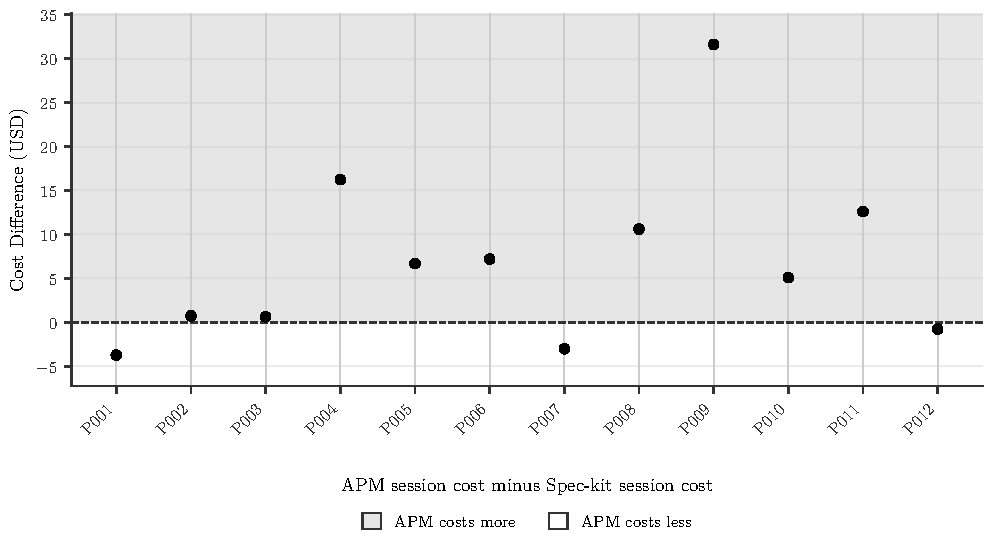
\includegraphics[width=0.85\textwidth]{figures/economic/cost_overall.pdf}
  \caption{Per-participant cost difference, APM minus Spec-kit, in US dollars. A point in the shaded region marks a participant for whom APM cost more.}
  \label{fig:cost-overall}
\end{figure}

The cost difference behaved very differently between the two model groups, set out in Table~\ref{tab:cost-model} and shown in Figure~\ref{fig:cost-by-model}. Among the participants who worked with Opus, five of the six APM sessions cost more, and the difference was large on all three summaries. The median and the Hodges-Lehmann estimate sit close together, with the mean a little above. Among the participants who worked with Sonnet the difference was small on all three summaries and mixed in direction, pointing to the two frameworks costing about the same for that group.

The Opus group also varied widely, from one session where APM cost about four dollars less to one where it cost about thirty-two dollars more. At six participants the confidence interval is wide and includes zero, with its bounds coinciding with those two extremes because at that sample size the interval reaches the smallest and largest differences rather than bounding the estimate more tightly. The Sonnet interval is similarly wide. Opus is the more expensive of the two models, so its differences fall on a larger dollar scale. Those large Opus values pulled the full-cohort summaries up, so the cohort-level cost difference comes mostly from the Opus group.

\begin{table}[H]
  \centering
  \caption{Paired cost differences within each model group, APM minus Spec-kit, in US dollars, at 96.9\% coverage.}
  \label{tab:cost-model}
  \begin{tabular}{lrrrrrr}
    \toprule
    Model & $n$ & Sign ($+$/$-$) & Median & HL & Mean & CI \\
    \midrule
    Opus & 6 & 5 / 1 & $+11.75$ & $+11.89$ & $+12.60$ & $[-3.73, +32.01]$ \\
    Sonnet & 6 & 4 / 2 & $+0.42$ & $+1.25$ & $+1.68$ & $[-2.72, +7.22]$ \\
    \bottomrule
  \end{tabular}
\end{table}

\begin{figure}[H]
  \centering
  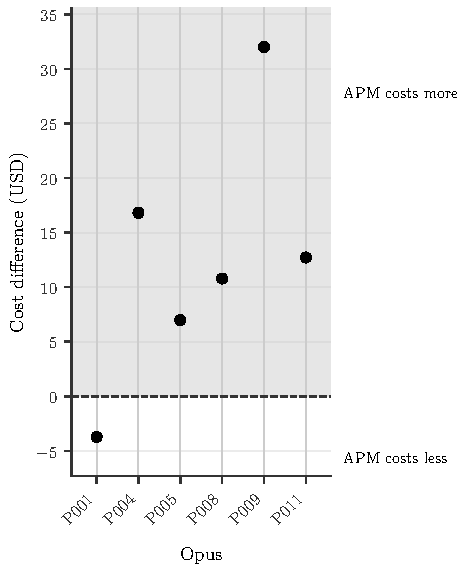
\includegraphics[width=0.49\textwidth]{figures/economic/cost_opus.pdf}\hfill
  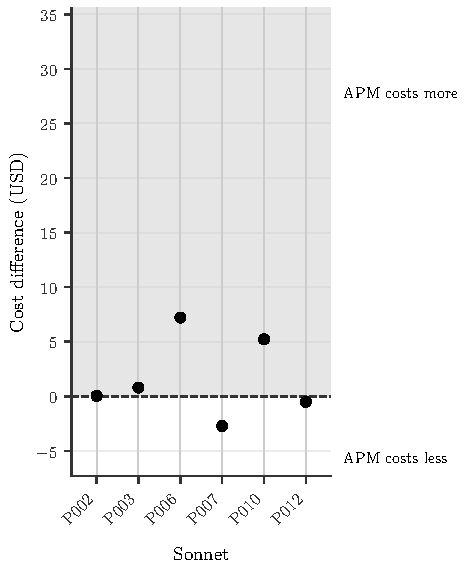
\includegraphics[width=0.49\textwidth]{figures/economic/cost_sonnet.pdf}
  \caption{Per-participant cost difference within each model, APM minus Spec-kit, in US dollars, on a shared scale.}
  \label{fig:cost-by-model}
\end{figure}

The two frameworks divided their spending differently across the task's two phases. As Table~\ref{tab:cost-phase} sets out, APM's planning phase cost less than Spec-kit's and its implementation phase cost more.\footnote{A small residual the parser records as an ``other'' phase, session activity outside either framework's workflow phases, accounts for under one percent of cost and a difference indistinguishable from zero, and is omitted.} Both phase differences exclude zero. The implementation excess was the larger of the two and set the direction of the overall difference. The pattern held in both models, stronger for the Opus group and slighter for the Sonnet group. The per-model split is given in Table~\ref{tab:cost-phase-model} in Appendix~\ref{app:cost-breakdowns}.

\begin{table}[H]
  \centering
  \caption{Paired cost differences by phase, APM minus Spec-kit, in US dollars, at 95.8\% coverage.}
  \label{tab:cost-phase}
  \begin{tabular}{lrrrrrr}
    \toprule
    Phase & $n$ & Sign ($+$/$-$) & Median & HL & Mean & CI \\
    \midrule
    Planning & 12 & 2 / 10 & $-3.77$ & $-4.89$ & $-5.17$ & $[-8.84, -1.44]$ \\
    Implementation & 12 & 10 / 2 & $+9.41$ & $+10.01$ & $+12.21$ & $[+4.10, +22.94]$ \\
    \bottomrule
  \end{tabular}
\end{table}

Within an APM session the cost divided across the three agent roles in the same shape under both models, as Table~\ref{tab:cost-role} details. The Planner and the Manager, the roles that plan the work and coordinate it rather than carry it out, cost on the same order as each other, each a fraction of the Worker's. The bulk of an APM session's cost therefore fell on the agents actually doing the implementation part of the implementation phase. Every role cost more under Opus than under Sonnet, matching the model's higher rate, while the order and rough proportions stayed the same.

\begin{table}[H]
  \centering
  \caption{Cost by agent role within the APM sessions, by model, in US dollars.}
  \label{tab:cost-role}
  \begin{tabular}{llrrr}
    \toprule
    Model & Role & Median & HL & Mean \\
    \midrule
    Opus & Planner & 5.50 & 5.85 & 6.53 \\
    Opus & Manager & 7.35 & 7.31 & 6.97 \\
    Opus & Worker & 21.76 & 21.80 & 22.91 \\
    Sonnet & Planner & 2.67 & 2.67 & 2.66 \\
    Sonnet & Manager & 2.68 & 2.68 & 2.62 \\
    Sonnet & Worker & 9.54 & 9.25 & 9.21 \\
    \bottomrule
  \end{tabular}
\end{table}

The cost difference also divides by token category, the kind of token each dollar paid for, as Table~\ref{tab:cost-token} reports. As Section~\ref{sec:context-windows-and-context-decay} described, each call reprocesses the whole session so far, and caching lowers the price of the tokens that repeat. Under both frameworks Claude Code caches almost all of that prompt, so uncached input was negligible, a few cents either way, and the framework's effect falls on the cache and output categories rather than on fresh input.

The two cache-write rows separate the main agents the user works in from the subagents those agents dispatch. Claude Code writes the one-hour cache for a main agent and the five-minute cache for a subagent. The one-hour writes therefore reflect the framework comparison most directly, since the framework sets how many main agents the user opens.

Two categories drove the difference: output and one-hour writes. APM produced more output than Spec-kit in all but one session and wrote more to the one-hour cache in every session, and for both categories the cohort confidence interval does not include zero. Both differences were larger under Opus than under Sonnet. The cache-read difference was mixed across the cohort, and its confidence interval includes zero. APM read more from the cache than Spec-kit under Opus, and less under Sonnet. The five-minute writes, the subagent cache, were a small positive difference. The per-model split of all five categories is given in Table~\ref{tab:cost-token-model} in Appendix~\ref{app:cost-breakdowns}.

\begin{table}[H]
  \centering
  \caption{Paired cost differences by token category, APM minus Spec-kit, in US dollars, at 95.8\% coverage.}
  \label{tab:cost-token}
  \begin{tabular}{lrrrrrr}
    \toprule
    Category & $n$ & Sign ($+$/$-$) & Median & HL & Mean & CI \\
    \midrule
    Input & 12 & 7 / 5 & $+0.00$ & $+0.00$ & $+0.01$ & $[-0.00, +0.01]$ \\
    Output & 12 & 11 / 1 & $+2.24$ & $+2.20$ & $+2.32$ & $[+1.15, +3.40]$ \\
    Cache read & 12 & 7 / 5 & $+1.16$ & $+1.20$ & $+1.82$ & $[-2.33, +6.03]$ \\
    Cache write (5-minute) & 12 & 10 / 2 & $+0.07$ & $+0.07$ & $+0.05$ & $[-0.00, +0.13]$ \\
    Cache write (1-hour) & 12 & 12 / 0 & $+2.67$ & $+2.50$ & $+2.92$ & $[+1.28, +4.65]$ \\
    \bottomrule
  \end{tabular}
\end{table}

Lastly, session order did not reverse the cost difference. APM cost more than Spec-kit whether participants met it first or second, in four of the six who used it first and five of the six who used it second. Table~\ref{tab:cost-order} in Appendix~\ref{app:cost-breakdowns} gives the difference within each order. The central difference was larger and more consistent when participants met APM second, but at six participants in each order the intervals are wide and the two orders cannot be told apart. The cost difference therefore tracks the framework rather than the order of the sessions, consistent with the learning-effects examination of Section~\ref{sec:disc-learning-effects}, which finds no measurable carry-over between a participant's two sessions.

Two sections in Chapter~\ref{chap:discussions} read these differences further. Section~\ref{sec:disc-sdd} traces the planning-phase difference to how the two frameworks carry out spec-driven planning. Section~\ref{sec:disc-cost-mechanics} takes up the implementation cost, how distributing the work across several agents shapes where the cost falls and why the two model groups diverge.

\section{Process}
\label{sec:results-process}

The process comparison reads how distributing the work across several agents changed the time each task took and the effort it asked of the user. The session's temporal shape is reported first, its interaction shape second.

\subsection{Temporal Shape}
\label{sec:results-process-time}

An APM session lasted a median of about 119 minutes against Spec-kit's 71, as Table~\ref{tab:proc-duration-fw} reports. APM's durations clustered tightly, with its Hodges-Lehmann estimate and mean close to the median, while Spec-kit's mean and Hodges-Lehmann estimate sat above its median, pulled up by a few long sessions. The two phases divided that time differently. APM's time fell mostly in implementation, at a median of about 77 minutes against Spec-kit's 30, while planning was closer and went the other way, with APM at about 36 minutes against Spec-kit's 49.

\begin{table}[H]
  \centering
  \caption{Per-framework session and phase durations, in seconds, across each framework's twelve sessions.}
  \label{tab:proc-duration-fw}
  \begin{tabular}{llrrr}
    \toprule
    Scope & Framework & Median & HL & Mean \\
    \midrule
    Session & APM & $7136.1$ & $7140.5$ & $7267.2$ \\
     & Spec-kit & $4274.6$ & $4684.6$ & $4810.2$ \\
    \midrule
    Planning & APM & $2153.4$ & $2179.3$ & $2298.9$ \\
     & Spec-kit & $2928.3$ & $2888.2$ & $2903.5$ \\
    \midrule
    Implementation & APM & $4641.5$ & $4790.6$ & $4865.1$ \\
     & Spec-kit & $1779.3$ & $1649.6$ & $1879.8$ \\
    \bottomrule
  \end{tabular}
\end{table}

APM was the longer session for every participant, as Table~\ref{tab:proc-time} reports. Paired within each participant, the difference came to a median of about 36 minutes, close to its Hodges-Lehmann estimate, and its confidence interval excludes zero. The session duration divides into the active turn time, when at least one agent was working, and the inter-turn idle between turns, and both were higher under APM in eleven of the twelve pairs.

\begin{table}[H]
  \centering
  \caption{Paired session-time differences across the cohort, APM minus Spec-kit, in seconds, at 95.8\% coverage. The turn time is the active span, and the inter-turn idle is the residual to the session duration.}
  \label{tab:proc-time}
  \begin{tabular}{lrrrrrr}
    \toprule
    Measure & $n$ & Sign ($+$/$-$) & Median & HL & Mean & CI \\
    \midrule
    Session duration & 12 & 12 / 0 & $+2160.7$ & $+2343.6$ & $+2457.0$ & $[+1394.2, +3594.2]$ \\
    Turn time & 12 & 11 / 1 & $+1834.7$ & $+1868.5$ & $+1860.4$ & $[+935.0, +2845.0]$ \\
    Inter-turn idle & 12 & 11 / 1 & $+674.4$ & $+650.1$ & $+596.7$ & $[+93.5, +1201.8]$ \\
    \bottomrule
  \end{tabular}
\end{table}

The session duration difference held under both models and was wider under Opus than Sonnet. Its split into active and idle time held under both as well, with the active-time gap the wider under Opus. Table~\ref{tab:proc-time-model} of Appendix~\ref{app:process-breakdowns} details the per-model split.

The two phases did not share that difference equally, as Table~\ref{tab:proc-phase} sets out. The implementation phase was longer under APM in every pair, with almost all of the extra time spent in active work, and it set the direction of the whole-session difference. The planning difference was a wash, mixed across participants with an interval spanning zero. The one clear planning contrast is in the active time, where Spec-kit's agent worked longer in eight of the twelve pairs, with an interval excluding zero, while the idle time between turns stood even between the frameworks.

\begin{table}[H]
  \centering
  \small
  \setlength{\tabcolsep}{4pt}
  \caption{Paired phase-time differences, APM minus Spec-kit, in seconds, at 95.8\% coverage. Each phase's duration divides into the active turn time and the inter-turn idle.}
  \label{tab:proc-phase}
  \begin{tabular}{llrrrrrr}
    \toprule
    Phase & Measure & $n$ & Sign ($+$/$-$) & Median & HL & Mean & CI \\
    \midrule
    Planning & Duration & 12 & 5 / 7 & $-539.2$ & $-611.9$ & $-604.6$ & $[-1382.7, +200.9]$ \\
     & Turn time & 12 & 4 / 8 & $-606.5$ & $-612.3$ & $-629.9$ & $[-1116.4, -49.1]$ \\
     & Inter-turn idle & 12 & 7 / 5 & $+98.6$ & $+102.3$ & $+25.2$ & $[-290.7, +314.4]$ \\
    \midrule
    Implementation & Duration & 12 & 12 / 0 & $+2549.0$ & $+2605.0$ & $+2985.3$ & $[+1711.9, +4384.1]$ \\
     & Turn time & 12 & 11 / 1 & $+2337.8$ & $+2357.6$ & $+2464.4$ & $[+1452.2, +3655.5]$ \\
     & Inter-turn idle & 12 & 9 / 3 & $+346.5$ & $+367.0$ & $+520.9$ & $[+59.4, +1095.0]$ \\
    \bottomrule
  \end{tabular}
\end{table}

Splitting the two phase differences by model changed neither result. Table~\ref{tab:proc-phase-model} of Appendix~\ref{app:process-breakdowns} presents the per-model view. The implementation phase was longer under APM in all six pairs of each model, with the typical difference somewhat larger under Sonnet. The planning difference remained mixed in sign under both models, with its interval spanning zero.

Session order did not reverse the duration difference. APM was the longer session in all six pairs whether participants met it first or second, as Table~\ref{tab:proc-order} of Appendix~\ref{app:process-breakdowns} reports. The central difference was somewhat larger when participants met APM first, but at six participants in each order the intervals are wide and the two orders cannot be told apart. The duration difference therefore tracks the framework rather than the order of the sessions.

Within the active time APM could have two or more of its agents working at once, which Spec-kit's single conversation cannot. The participants made little use of it. The agents worked one at a time in five of the twelve sessions, and in the seven where they overlapped the concurrent span was a small part of the active time. Table~\ref{tab:proc-concurrency} in Appendix~\ref{app:process-breakdowns} gives the per-session split.

Figure~\ref{fig:proc-temporal} shows each participant's two sessions as paired bars. The filled lower part of each bar is the active time and the open upper part the idle time, so the full height is the session duration. APM's bars stand taller across the cohort, with its active time consistently larger than its Spec-kit pair.

\begin{figure}[H]
  \centering
  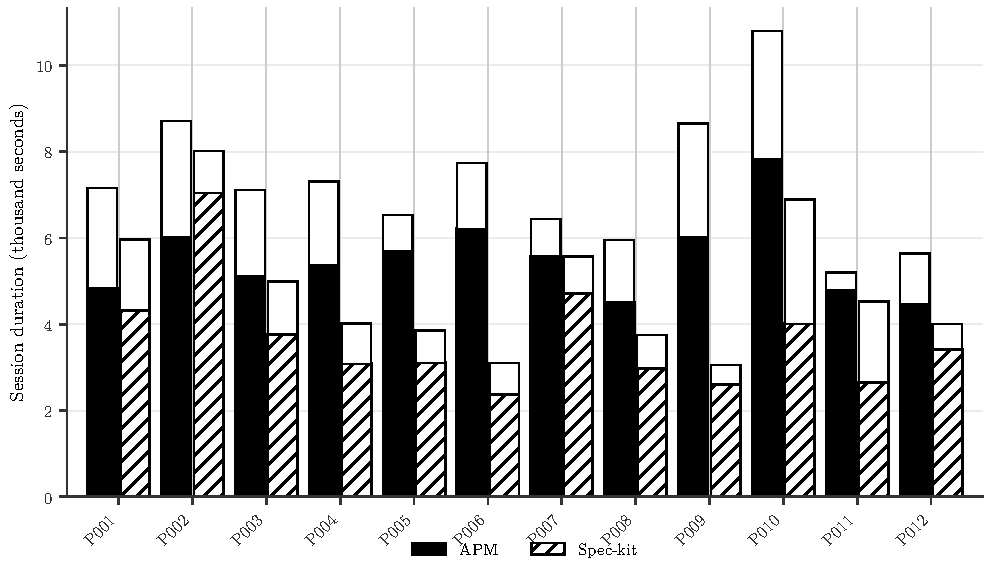
\includegraphics[width=0.85\textwidth]{figures/process/temporal.pdf}
  \caption{Per-participant session temporal shape. Each participant has two bars, APM and Spec-kit; the filled lower segment is the active time, the open upper segment the inter-turn idle, and the full height the session duration.}
  \label{fig:proc-temporal}
\end{figure}

\subsection{Interaction Shape}
\label{sec:results-process-interaction}

\placeholder{Forthcoming. The turn-prompt count compared between frameworks, at the session scope and split by phase, with each framework's typical level reported alongside the paired difference. The per-framework composition of the user's messages across the protocol, short, and standard buckets, by phase, with the mean character length per bucket. The role distribution of the turn prompts across APM's agents. Steering reported as a brief aside. Per-model and per-order breakdowns and the per-participant distributions are deferred to Appendix~\ref{app:process-breakdowns}.}

\section{Functional}
\label{sec:results-functional}

\placeholder{Forthcoming. The total rubric score compared between frameworks by the paired method of the Analysis Plan, the per-section scores decomposing it across the Python and C implementations, and the per-framework score distribution with every session shown. The perceived-effectiveness rating from the questionnaire is reported alongside.}

\section{Perception}
\label{sec:results-perception}

\placeholder{Forthcoming. The eight ordinal rating items compared between frameworks item by item, each by its sign count and median paired difference read with the item's polarity, with the per-framework median profile across the items; the second-session comparative item reported by the framework taken second. Each rating is read against the behaviour it should reflect, descriptively, as the pattern of agreement and divergence.}

\section{Supplementary}
\label{sec:results-supplementary}

\placeholder{Forthcoming. Descriptive per-framework summaries for the supplementary measures: tool success rate, subagent dispatch count, delegated tool-use count, and model-invoked Skill count, per framework and per model, descriptive only and without a paired comparison.}



\chapter{DISCUSSION}
\label{chap:discussion}
% Discussions chapter body. Included by thesis.tex under \chapter{DISCUSSIONS}.
% This is an \input fragment, not a standalone document.

\placeholder{Forthcoming. Interpretation of the results, reading the framework comparison across the economic, process, functional, and perception dimensions against the structure and design of the two frameworks. The subsections below are themed to the deeper questions each results section raises.}

\section{Two Realisations of Spec-Driven Development}
\label{sec:disc-sdd}

Spec-kit's planning phase cost more than APM's in ten of the twelve pairs, the one part of the task where APM was the cheaper of the two, as the planning row of Table~\ref{tab:cost-phase} records. The difference follows from how each framework carries out the planning of spec-driven development. Spec-kit plans more autonomously, having the agent explore the codebase and, on ambiguities, decide on best practices, drawing on the model's capabilities and training data. It fills a fixed set of template documents from what it finds, putting few or no questions to the user. APM explores the codebase as well, but it leans more on the user's input and builds review checkpoints into its planning. Required rounds of questions keep the user engaged and abreast of the planning. From what they supply, APM writes three shorter documents that generalise across project types. The two approaches are set out where each framework is introduced, Spec-kit in Section~\ref{sec:frameworks-under-comparison} and APM in Chapter~\ref{chap:framework-design}.

The cost gap has two drivers visible in the planning phase, both pointing the same way, set out in Table~\ref{tab:planning-behaviour}. Spec-kit issued more requests to the model in every one of the twelve pairs, around thirty-nine more at the median and near fifty-seven by the Hodges-Lehmann estimate, with a few pairs where the gap ran much wider. These are the extra steps of an agent that explores and drafts without waiting on the user. Spec-kit also produced more output in nine of the twelve pairs, about thirty-four thousand tokens more at the median and near thirty-six thousand by the Hodges-Lehmann estimate, the text that fills its larger set of documents. APM ran lighter on both.

\begin{table}[H]
  \centering
  \caption{Paired planning-phase request and output differences, APM minus Spec-kit, at 95.8\% coverage.}
  \label{tab:planning-behaviour}
  \begin{tabular}{lrrrrrr}
    \toprule
    Measure & $n$ & Sign ($+$/$-$) & Median & HL & Mean & CI \\
    \midrule
    Requests & 12 & 0 / 12 & $-38.5$ & $-56.5$ & $-60.7$ & $[-95.0, -29.0]$ \\
    Output (thousand tokens) & 12 & 3 / 9 & $-34.5$ & $-35.7$ & $-39.7$ & $[-70.5, -9.9]$ \\
    \bottomrule
  \end{tabular}
\end{table}

The difference is larger under Opus and smaller under Sonnet, yet points the same way in both model groups, as the per-model split in Table~\ref{tab:planning-behaviour-model} of Appendix~\ref{app:sdd-breakdowns} sets out. Spec-kit's heavier request count holds in every pair under both, and its larger output is present in both as well. The typical sizes widen under Opus. With six participants in each group the per-model intervals are wide, so the pooled comparison carries the statistical weight.

In implementation the two frameworks converge. Both build against the planning documents as the source of truth and revise them as findings require, differing in the detail but not the essence. They part on cost. It is there that APM costs more, and that excess is the larger part of the overall difference, coming from how APM splits the work across several agents rather than from how it plans. Section~\ref{sec:disc-cost-mechanics} takes that up.

\placeholder{Forthcoming. The process reading of this realisation: how Spec-kit's autonomous planning shows in the planning phase's turn count and turn time, the more self-driven turns taken over a longer span, set against the lighter user-involved planning of APM.}

\placeholder{Forthcoming. The functional reading of this realisation: the failures connected to how each framework planned, read by their size and type.}

\placeholder{Forthcoming. The perception reading of this realisation, how the two planning approaches relate to what participants reported.}

\section{Cost Mechanics of APM and Spec-kit}
\label{sec:disc-cost-mechanics}

\placeholder{Forthcoming. The implementation-phase cost of each framework and what drives it, including how APM distributes the work across several agents and why the two models diverge.}

\section{Learning Effects}
\label{sec:disc-learning-effects}

The confined number of sessions in the case study allows each participant's pair to be examined individually for learning carried from the first session into the second. The workspace and the agent are reset between sessions, so the participant is the only carrier of that memory, and the evidence is sought in their own inputs: a second-session instruction that pre-empts an error the first session made, an explicit reference to an earlier decision, or a detail handled correctly from recall rather than rediscovered. A stronger second-session result alone does not count, since the agent may have produced it unaided. These signs are read case by case, as indications of learning rather than a conclusive measure of it.

\placeholder{Forthcoming. The per-participant verdicts on carried-over learning and the cohort read drawn from them.}

\section{Threats to Validity}
\label{sec:threats}

This section enumerates the internal, external, and construct validity threats and the mitigations applied. Each threat points back to the specific section that motivates it.

\subsection{Internal Validity}

\textbf{Learning effects from the within-subjects design.} The within-subjects design declared in the Case-Study Design (Section~\ref{sec:case-study-design}) has each participant complete the same task twice, so task familiarity from the first session can influence performance in the second. Counterbalancing the framework order across participants, as described in Sessions and Data (Section~\ref{sec:sessions-data}), mitigates the framework-effect confound but does not eliminate the underlying learning curve. The learning-effects examination described in Section~\ref{sec:disc-learning-effects} reads each participant's two sessions for evidence of carried-over learning and is the primary defence against this threat.

\textbf{Self-reported versus observed measures.} The perception measures described in Section~\ref{sec:measures} pair the instrumented, transcript-derived measures with self-reported workload, confidence, and perceived framework effectiveness; observed divergences between self-report and instrument are reported as findings rather than absorbed as an unstated limitation. Residual risk remains: self-reports are subject to recall bias and social-desirability pressures that the instrument-side measurements cannot independently correct.

\subsection{External Validity}

\textbf{Generalisation scope.} The case study is run on a single AI coding CLI, against a complex software engineering task requiring two-language implementation and legacy-codebase research, described in the Task Specification (Section~\ref{sec:task-spec}), in a setting positioned between laboratory and field conditions. Findings generalise within this scope and do not generalise to multi-platform settings, dynamic cross-model routing, simpler or less knowledge-intensive tasks, or pure laboratory or natural-setting conditions.

\textbf{Temporal decay of findings.} The AI coding assistant field is evolving rapidly. Effect sizes and descriptive claims throughout this chapter (rate-card prices, command sets, framework releases, and model availability) are tied to the May 2026 snapshot stated in Section~\ref{sec:methodology}. The dollar-equivalent cost values reported under Chapter~\ref{chap:results} rest on the rate-card snapshot; results that rest on those specific rates are defensible against the snapshot but may require re-estimation under a materially different rate card.

\subsection{Construct Validity}

\textbf{Behavioural input buckets as process-efficiency proxy.} The short, protocol, and standard input buckets defined under the Process measures in Section~\ref{sec:measures} are extracted from the transcript content for this study. They are not validated against an external coordination-burden instrument. Their validity as proxies for human coordination effort rests on face validity alone: the relative ordering of frameworks along these metrics is robust, but the absolute magnitude of differences is interpretive rather than calibrated.

\textbf{Instrument coverage limits.} The 100-point rubric captures correctness and robustness but not code quality, maintainability, security posture, or long-term technical debt. Metric extraction is further limited to the Claude Code JSONL transcripts and their sibling subagent files that accompany each participant submission, as declared in Sessions and Data (Section~\ref{sec:sessions-data}): any interaction with the AI that took place outside the CLI's transcript surface is invisible to the metric set.

\textbf{Replica versus live Open eClass.} The shared Docker-based replica of the Open eClass platform described in the Task Environment (Section~\ref{sec:task-env}) pins the platform to a fixed upstream baseline and seeds deterministic fixture data. The shared replica makes the cohort comparable and the grading reproducible, and removes any parity gap between what participants build against and what the evaluation runs against. The trade-off is that the task is performed against a replica rather than against any live university instance of Open eClass: any property of a live instance that the replica does not reproduce, such as timezone handling of locale-formatted dates, session-cookie behaviour under load, cross-origin interactions with the mock CAS service, or upstream behaviours that have shifted since the baseline commit, is not exercised by the case study.


\chapter{CONCLUSION}
\label{chap:conclusion}
% !TEX root = ../../thesis.tex
% Conclusion chapter body. Included by thesis.tex under \chapter{CONCLUSION}.

\placeholder{Forthcoming. Restate the proposition and how the evidence bears
on it; limitations (pointer to the Threats subsection); and Future Work as the
closing section.}


\backmatter

\abbreviations

\begin{longtable}{@{}l@{\hspace{2em}}p{0.72\textwidth}@{}}
  \toprule
  Abbreviation & Meaning \\
  \midrule
  \endfirsthead
  \toprule
  Abbreviation & Meaning \\
  \midrule
  \endhead
  \bottomrule
  \endlastfoot
  AI       & Artificial Intelligence \\
  API      & Application Programming Interface \\
  APM      & Agentic Project Management \\
  CI       & Confidence Interval \\
  HL       & Hodges-Lehmann estimate \\
  JSON     & JavaScript Object Notation \\
  JSON-RPC & JSON Remote Procedure Call \\
  LLM      & Large Language Model \\
  MAS      & Multi-Agent System \\
  MCP      & Model Context Protocol \\
  PHP      & PHP: Hypertext Preprocessor \\
  PRD      & Product Requirements Document \\
  RQ       & Research Question \\
  SDD      & Spec-Driven Development \\
  SDK      & Software Development Kit \\
  TDD      & Test-Driven Development \\
  YAML     & YAML Ain't Markup Language \\
\end{longtable}

\begin{appendix}
\appendixstartedtrue
\phantomsection
\addcontentsline{toc}{chapter}{APPENDICES}

\chapter{EVALUATION APPENDIX}
% Evaluation appendix body. Included by thesis.tex under
% \chapter{EVALUATION APPENDIX} inside the \appendix block.

\section{Rate Card}
\label{app:rate-card}

The dollar-equivalent cost prices each call's tokens at the rates in Table~\ref{tab:rate-card}. The rates cover five token categories, fresh input and output, reads from the prompt cache, and writes to the cache at its five-minute and one-hour retention tiers.

\begin{table}[ht]
  \centering
  \caption{Per-token rates for the study window, in US dollars per million tokens.}
  \label{tab:rate-card}
  \begin{tabular}{lrrrrr}
    \toprule
    Model & Input & Output & Cache read & Cache write (5\,min) & Cache write (1\,h) \\
    \midrule
    Opus 4.7 & 5.00 & 25.00 & 0.50 & 6.25 & 10.00 \\
    Sonnet 4.6 & 3.00 & 15.00 & 0.30 & 3.75 & 6.00 \\
    Haiku 4.5 & 1.00 & 5.00 & 0.10 & 1.25 & 2.00 \\
    \bottomrule
  \end{tabular}
\end{table}

Although a participant's assigned model was fixed to Opus 4.7 or Sonnet 4.6 for the agents they used, the subagents those agents dispatch and some background operations were at times routed to Haiku, so some sessions carry a small share of Haiku tokens alongside their assigned model. The rates are held as a data file, \texttt{rates.yaml}, in the evaluation infrastructure.\footnote{Available at: \url{https://github.com/sdi2200262/bsc-apm-case-study-infra}}


\chapter{RESULTS APPENDIX}
% Results appendix body. Included by thesis.tex under
% \chapter{RESULTS APPENDIX} inside the \appendix block.

\section{Economic Cost Breakdowns}
\label{app:cost-breakdowns}

These tables give the per-model and per-order detail behind claims in the Economic results (Section~\ref{sec:results-economic}).

Table~\ref{tab:cost-phase-model} splits the phase cost difference by model. The split is wider under Opus.

\begin{table}[H]
  \centering
  \caption{Paired cost differences by phase within each model, APM minus Spec-kit, in US dollars, at 96.9\% coverage.}
  \label{tab:cost-phase-model}
  \begin{tabular}{llrrrrrr}
    \toprule
    Model & Phase & $n$ & Sign ($+$/$-$) & Median & HL & Mean & CI \\
    \midrule
    Opus & Planning & 6 & 1 / 5 & $-5.38$ & $-6.64$ & $-6.92$ & $[-14.25, +0.55]$ \\
    Opus & Implementation & 6 & 6 / 0 & $+15.71$ & $+18.30$ & $+19.39$ & $[+2.08, +46.26]$ \\
    Sonnet & Planning & 6 & 1 / 5 & $-1.64$ & $-2.89$ & $-3.41$ & $[-11.29, +0.28]$ \\
    Sonnet & Implementation & 6 & 4 / 2 & $+4.48$ & $+4.48$ & $+5.03$ & $[-0.38, +13.26]$ \\
    \bottomrule
  \end{tabular}
\end{table}

Table~\ref{tab:cost-token-model} splits the token-category cost difference by model. The output and one-hour cache-write differences are larger under Opus, and the cache-read difference reverses sign between the models.

\begin{table}[H]
  \centering
  \small
  \caption{Paired cost differences by token category within each model, APM minus Spec-kit, in US dollars, at 96.9\% coverage.}
  \label{tab:cost-token-model}
  \begin{tabular}{llrrrrrr}
    \toprule
    Model & Category & $n$ & Sign ($+$/$-$) & Median & HL & Mean & CI \\
    \midrule
    Opus & Input & 6 & 5 / 1 & $+0.00$ & $+0.00$ & $+0.01$ & $[-0.01, +0.06]$ \\
    Opus & Output & 6 & 5 / 1 & $+3.28$ & $+3.20$ & $+3.10$ & $[-0.07, +6.12]$ \\
    Opus & Cache read & 6 & 5 / 1 & $+3.51$ & $+4.91$ & $+4.73$ & $[-7.30, +17.12]$ \\
    Opus & Cache write (5-minute) & 6 & 6 / 0 & $+0.07$ & $+0.08$ & $+0.09$ & $[+0.00, +0.24]$ \\
    Opus & Cache write (1-hour) & 6 & 6 / 0 & $+3.72$ & $+4.51$ & $+4.67$ & $[+2.92, +8.53]$ \\
    \midrule
    Sonnet & Input & 6 & 2 / 4 & $-0.00$ & $+0.00$ & $+0.00$ & $[-0.00, +0.01]$ \\
    Sonnet & Output & 6 & 6 / 0 & $+1.30$ & $+1.58$ & $+1.56$ & $[+0.66, +2.80]$ \\
    Sonnet & Cache read & 6 & 2 / 4 & $-1.34$ & $-1.34$ & $-1.08$ & $[-5.74, +1.94]$ \\
    Sonnet & Cache write (5-minute) & 6 & 4 / 2 & $+0.07$ & $+0.05$ & $+0.02$ & $[-0.29, +0.14]$ \\
    Sonnet & Cache write (1-hour) & 6 & 6 / 0 & $+1.12$ & $+1.12$ & $+1.18$ & $[+0.20, +2.41]$ \\
    \bottomrule
  \end{tabular}
\end{table}

Table~\ref{tab:cost-order} splits the cost difference by the order in which the participant met the two frameworks. The central difference was larger when APM came second, but with six participants in each order the intervals are wide and the two orders are not distinguishable.

\begin{table}[H]
  \centering
  \caption{Paired cost differences by session order, APM minus Spec-kit, in US dollars, at 96.9\% coverage.}
  \label{tab:cost-order}
  \begin{tabular}{lrrrrrr}
    \toprule
    Order & $n$ & Sign ($+$/$-$) & Median & HL & Mean & CI \\
    \midrule
    APM first & 6 & 4 / 2 & $+3.89$ & $+3.89$ & $+6.76$ & $[-3.73, +32.01]$ \\
    APM second & 6 & 5 / 1 & $+8.01$ & $+8.01$ & $+7.51$ & $[-0.51, +16.81]$ \\
    \bottomrule
  \end{tabular}
\end{table}

\newpage
\section{Process Breakdowns}
\label{app:process-breakdowns}

These tables give the per-model and per-order breakdowns, and the per-session active-time composition, behind claims in the Process results (Section~\ref{sec:results-process}).

Table~\ref{tab:proc-time-model} gives the session-time differences within each model group, the per-model split of Table~\ref{tab:proc-time}. APM was higher on the session duration in all six pairs under each model, with the gap the wider under Opus, and its active and idle components were higher under APM in each group as well.

\begin{table}[H]
  \centering
  \small
  \setlength{\tabcolsep}{4pt}
  \caption{Paired session-time differences within each model group, APM minus Spec-kit, in seconds, at 96.9\% coverage. The measures are those of Table~\ref{tab:proc-time}.}
  \label{tab:proc-time-model}
  \begin{tabular}{llrrrrrr}
    \toprule
    Model & Measure & $n$ & Sign ($+$/$-$) & Median & HL & Mean & CI \\
    \midrule
    Opus & Session duration & 6 & 6 / 0 & $+2436.4$ & $+2436.4$ & $+2603.4$ & $[+664.1, +5596.1]$ \\
     & Turn time & 6 & 6 / 0 & $+2206.9$ & $+2139.4$ & $+2076.9$ & $[+519.7, +3415.5]$ \\
     & Inter-turn idle & 6 & 5 / 1 & $+674.4$ & $+667.1$ & $+526.5$ & $[-1475.3, +2180.6]$ \\
    \midrule
    Sonnet & Session duration & 6 & 6 / 0 & $+1878.6$ & $+2302.2$ & $+2310.7$ & $[+701.8, +4635.4]$ \\
     & Turn time & 6 & 5 / 1 & $+1199.3$ & $+1384.4$ & $+1643.8$ & $[-1034.8, +3833.9]$ \\
     & Inter-turn idle & 6 & 6 / 0 & $+679.3$ & $+679.3$ & $+666.9$ & $[+5.8, +1736.6]$ \\
    \bottomrule
  \end{tabular}
\end{table}

Table~\ref{tab:proc-phase-model} splits the phase-time differences by model, the per-model view of Table~\ref{tab:proc-phase}. The implementation phase was longer under APM in all six pairs of each model, with the difference somewhat larger under Sonnet, while the planning difference remained mixed in sign under both.

\begin{table}[H]
  \centering
  \small
  \setlength{\tabcolsep}{3pt}
  \caption{Paired phase-time differences within each model group, APM minus Spec-kit, in seconds, at 96.9\% coverage. Each phase's duration divides into the active turn time and the inter-turn idle.}
  \label{tab:proc-phase-model}
  \begin{tabular}{lllrrrrrr}
    \toprule
    Model & Phase & Measure & $n$ & Sign ($+$/$-$) & Median & HL & Mean & CI \\
    \midrule
    Opus & Planning & Duration & 6 & 3 / 3 & $-411.0$ & $-600.3$ & $-549.2$ & $[-1963.8, +763.3]$ \\
     & & Turn time & 6 & 3 / 3 & $-331.3$ & $-532.3$ & $-502.9$ & $[-1429.8, +139.3]$ \\
     & & Inter-turn idle & 6 & 3 / 3 & $+112.2$ & $+39.6$ & $-46.3$ & $[-1223.4, +642.0]$ \\
     & Implementation & Duration & 6 & 6 / 0 & $+2339.0$ & $+2339.0$ & $+3039.1$ & $[+1778.6, +7287.3]$ \\
     & & Turn time & 6 & 6 / 0 & $+2337.8$ & $+2337.8$ & $+2557.4$ & $[+1452.2, +4845.3]$ \\
     & & Inter-turn idle & 6 & 4 / 2 & $+247.9$ & $+247.9$ & $+481.6$ & $[-252.0, +2442.0]$ \\
    \midrule
    Sonnet & Planning & Duration & 6 & 2 / 4 & $-539.2$ & $-649.6$ & $-660.1$ & $[-2404.0, +821.2]$ \\
     & & Turn time & 6 & 1 / 5 & $-637.8$ & $-765.5$ & $-756.8$ & $[-2043.1, +308.5]$ \\
     & & Inter-turn idle & 6 & 4 / 2 & $+98.6$ & $+98.6$ & $+96.8$ & $[-360.8, +512.7]$ \\
     & Implementation & Duration & 6 & 6 / 0 & $+2878.6$ & $+2878.6$ & $+2931.5$ & $[+589.7, +6046.7]$ \\
     & & Turn time & 6 & 5 / 1 & $+2363.8$ & $+2363.8$ & $+2371.4$ & $[-858.7, +5188.8]$ \\
     & & Inter-turn idle & 6 & 5 / 1 & $+514.8$ & $+514.8$ & $+560.1$ & $[-47.1, +1448.4]$ \\
    \bottomrule
  \end{tabular}
\end{table}

Table~\ref{tab:proc-order} gives the session-duration difference within each session order. Neither order reverses it, with the central difference somewhat larger when APM came first.

\begin{table}[H]
  \centering
  \caption{Paired session-duration differences by session order, APM minus Spec-kit, in seconds, at 96.9\% coverage.}
  \label{tab:proc-order}
  \begin{tabular}{lrrrrrr}
    \toprule
    Order & $n$ & Sign ($+$/$-$) & Median & HL & Mean & CI \\
    \midrule
    APM first & 6 & 6 / 0 & $+2400.0$ & $+2751.4$ & $+2850.1$ & $[+867.4, +5596.1]$ \\
    APM second & 6 & 6 / 0 & $+1915.0$ & $+1993.8$ & $+2064.0$ & $[+664.1, +3902.6]$ \\
    \bottomrule
  \end{tabular}
\end{table}

Table~\ref{tab:proc-concurrency} sets out the active-time composition of each APM session, the solo and concurrent spans behind the concurrency reading in Section~\ref{sec:results-process-time}. The concurrent span was negligible in five of the twelve sessions and under a sixth of the active time in all but one.

\begin{table}[H]
  \centering
  \caption{Active-time composition of the APM sessions, in seconds, with the concurrent span as a share of the active time. Descriptive and APM only, since Spec-kit's single conversation has no concurrent span.}
  \label{tab:proc-concurrency}
  \begin{tabular}{lrrr}
    \toprule
    Participant & Solo & Concurrent & Concurrent share \\
    \midrule
    P001 & 4834 & 0 & 0.0\% \\
    P002 & 5993 & 16 & 0.3\% \\
    P003 & 4458 & 661 & 12.9\% \\
    P004 & 5300 & 58 & 1.1\% \\
    P005 & 5686 & 0 & 0.0\% \\
    P006 & 6203 & 9 & 0.1\% \\
    P007 & 4765 & 812 & 14.6\% \\
    P008 & 3934 & 580 & 12.8\% \\
    P009 & 4476 & 1541 & 25.6\% \\
    P010 & 6556 & 1259 & 16.1\% \\
    P011 & 4218 & 577 & 12.0\% \\
    P012 & 4037 & 429 & 9.6\% \\
    \bottomrule
  \end{tabular}
\end{table}

% Interaction Shape appendix entries: cleared for rewrite.


\end{appendix}

\printbibliography[title={BIBLIOGRAPHY}]

\end{document}
